\documentclass{standalone}

\usepackage{mathtools,pgfplots}
\pgfplotsset{compat=newest}

\let\Im\relax
\DeclareMathOperator{\Im}{Im}
\let\Re\relax
\DeclareMathOperator{\Re}{Re}

\begin{document}
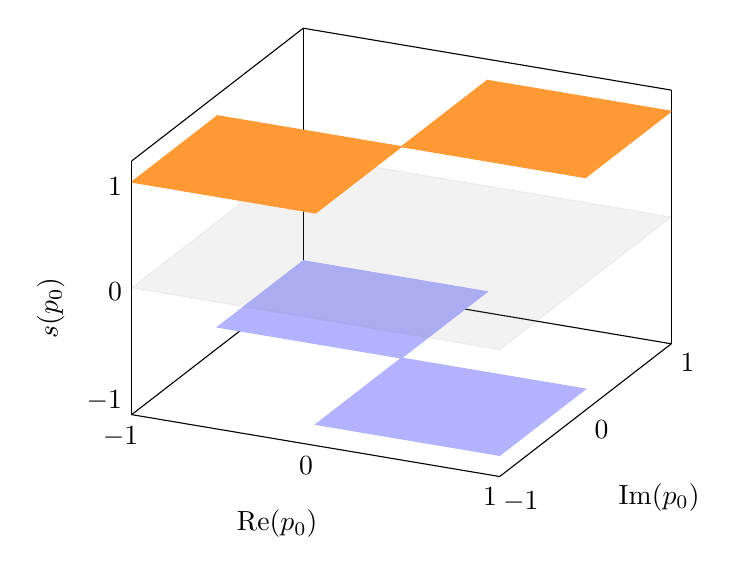
\begin{tikzpicture}
  \begin{axis}[
      xlabel=$\Re(p_0)$,
      ylabel=$\Im(p_0)$,
      zlabel=$s(p_0)$,
      domain=-1:1, surf, shader=flat,
      xtick distance=1,
      ytick distance=1,
      ztick distance=1,
      tickwidth=0,
    ]

    \addplot3[blue!30] coordinates {
        (-1, 1, -1) (0, 1, -1)

        (-1, 0, -1) (0, 0, -1)
      };

    \addplot3[blue!30] coordinates {
        (1, -1, -1) (0, -1, -1)

        (1, 0, -1) (0, 0, -1)
      };

    % Zero plane
    \addplot3[gray, opacity=0.1, samples=2]{0};

    \addplot3[orange!80] coordinates {
        (0, 0, 1) (1, 0, 1)

        (0, 1, 1) (1, 1, 1)
      };

    \addplot3[orange!80] coordinates {
        (0, 0, 1) (-1, 0, 1)

        (0, -1, 1) (-1, -1, 1)
      };

  \end{axis}
\end{tikzpicture}
\end{document}
